\documentclass{standalone}
\usepackage[T1]{fontenc}
\renewcommand*\familydefault{\sfdefault} %%
\usepackage{sfmath}
\usepackage{pgfplots}

\begin{document}



\tikzset{every picture/.style={line width=0.75pt}} %set default line width to 0.75pt        

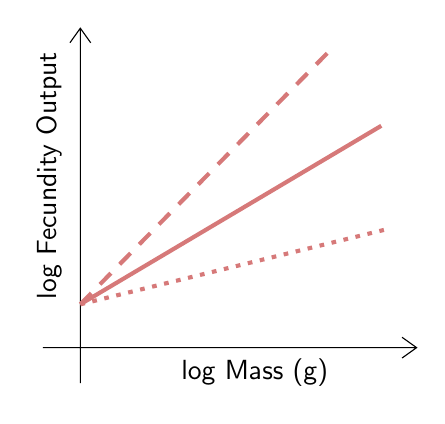
\begin{tikzpicture}[x=0.75pt,y=0.75pt,yscale=-1,xscale=1]
%uncomment if require: \path (0,300); %set diagram left start at 0, and has height of 300

%Shape: Axis 2D [id:dp048267521500923394] 
\draw  (146,210.9) -- (326,210.9)(164,57) -- (164,228) (319,205.9) -- (326,210.9) -- (319,215.9) (159,64) -- (164,57) -- (169,64)  ;
%Straight Lines [id:da2696070787992928] 
\draw [color={rgb, 255:red, 214; green, 121; blue, 121 }  ,draw opacity=1 ][line width=1.5]    (164,190) -- (309,104) ;


%Straight Lines [id:da7722707394287434] 
\draw [color={rgb, 255:red, 214; green, 121; blue, 121 }  ,draw opacity=1 ][line width=1.5]  [dash pattern={on 5.63pt off 4.5pt}]  (164,190) -- (283,69) ;


%Straight Lines [id:da656860480288004] 
\draw [color={rgb, 255:red, 214; green, 121; blue, 121 }  ,draw opacity=1 ][line width=1.5]  [dash pattern={on 1.69pt off 2.76pt}]  (164,190) -- (311,154) ;



% Text Node
\draw (149,128) node [rotate=-270] [align=left] {log Fecundity Output};
% Text Node
\draw (248,223) node  [align=left] {log Mass (g)};


\end{tikzpicture}

\end{document}